% Options for packages loaded elsewhere
\PassOptionsToPackage{unicode}{hyperref}
\PassOptionsToPackage{hyphens}{url}
%
\documentclass[
]{article}
\usepackage{lmodern}
\usepackage{amssymb,amsmath}
\usepackage{ifxetex,ifluatex}
\ifnum 0\ifxetex 1\fi\ifluatex 1\fi=0 % if pdftex
  \usepackage[T1]{fontenc}
  \usepackage[utf8]{inputenc}
  \usepackage{textcomp} % provide euro and other symbols
\else % if luatex or xetex
  \usepackage{unicode-math}
  \defaultfontfeatures{Scale=MatchLowercase}
  \defaultfontfeatures[\rmfamily]{Ligatures=TeX,Scale=1}
\fi
% Use upquote if available, for straight quotes in verbatim environments
\IfFileExists{upquote.sty}{\usepackage{upquote}}{}
\IfFileExists{microtype.sty}{% use microtype if available
  \usepackage[]{microtype}
  \UseMicrotypeSet[protrusion]{basicmath} % disable protrusion for tt fonts
}{}
\makeatletter
\@ifundefined{KOMAClassName}{% if non-KOMA class
  \IfFileExists{parskip.sty}{%
    \usepackage{parskip}
  }{% else
    \setlength{\parindent}{0pt}
    \setlength{\parskip}{6pt plus 2pt minus 1pt}}
}{% if KOMA class
  \KOMAoptions{parskip=half}}
\makeatother
\usepackage{xcolor}
\IfFileExists{xurl.sty}{\usepackage{xurl}}{} % add URL line breaks if available
\IfFileExists{bookmark.sty}{\usepackage{bookmark}}{\usepackage{hyperref}}
\hypersetup{
  hidelinks,
  pdfcreator={LaTeX via pandoc}}
\urlstyle{same} % disable monospaced font for URLs
\usepackage[margin=1in]{geometry}
\usepackage{graphicx}
\makeatletter
\def\maxwidth{\ifdim\Gin@nat@width>\linewidth\linewidth\else\Gin@nat@width\fi}
\def\maxheight{\ifdim\Gin@nat@height>\textheight\textheight\else\Gin@nat@height\fi}
\makeatother
% Scale images if necessary, so that they will not overflow the page
% margins by default, and it is still possible to overwrite the defaults
% using explicit options in \includegraphics[width, height, ...]{}
\setkeys{Gin}{width=\maxwidth,height=\maxheight,keepaspectratio}
% Set default figure placement to htbp
\makeatletter
\def\fps@figure{htbp}
\makeatother
\setlength{\emergencystretch}{3em} % prevent overfull lines
\providecommand{\tightlist}{%
  \setlength{\itemsep}{0pt}\setlength{\parskip}{0pt}}
\setcounter{secnumdepth}{-\maxdimen} % remove section numbering

\author{}
\date{\vspace{-2.5em}}

\begin{document}

\hypertarget{intro}{%
\section{Introduction}\label{intro}}

The introduction should provide an overview of the work you set out to
do and provide structure for the remainder of the document.

\hypertarget{background}{%
\subsection{Background}\label{background}}

\begin{itemize}
\item
  (coal ash report - car) coal one of the most dangerous combustible
  fossil fuels is comprised of a long list of dangerous chemicals --
  including substances such as arsenic, radium, other carcinogens,
  metals that can impair developing children's brains, toxins dangerous
  to aquatic life, etc {[}@Kelderman2019{]}
\item
  power plants produce 100mil tons of coal ash every year, which is
  dumped into landfills and waste ponds {[}@Kelderman2019{]}
\item
  only recently (2015) have complaints and lawsuit arisen in which
  certain ecological organizations have attempted to sue the EPA to
  regulate disposal of coal ash {[}@Kelderman2019{]}
\item
  this coal ash rule has forced power companies to make publicly
  available data regarding chemical concentrations in 265 coal plants
  containing ponds and landfills (about 3/4 of all coal power plants
  across the US) {[}@Kelderman2019{]}
\item
  environmental agencies have concluded that the groundwater under
  basically all coal plants are contaminated {[}@Kelderman2019{]}
\item
  HOWEVER this might be overstated? we wanted to investigate whether or
  not if this was true.
\end{itemize}

\begin{figure}
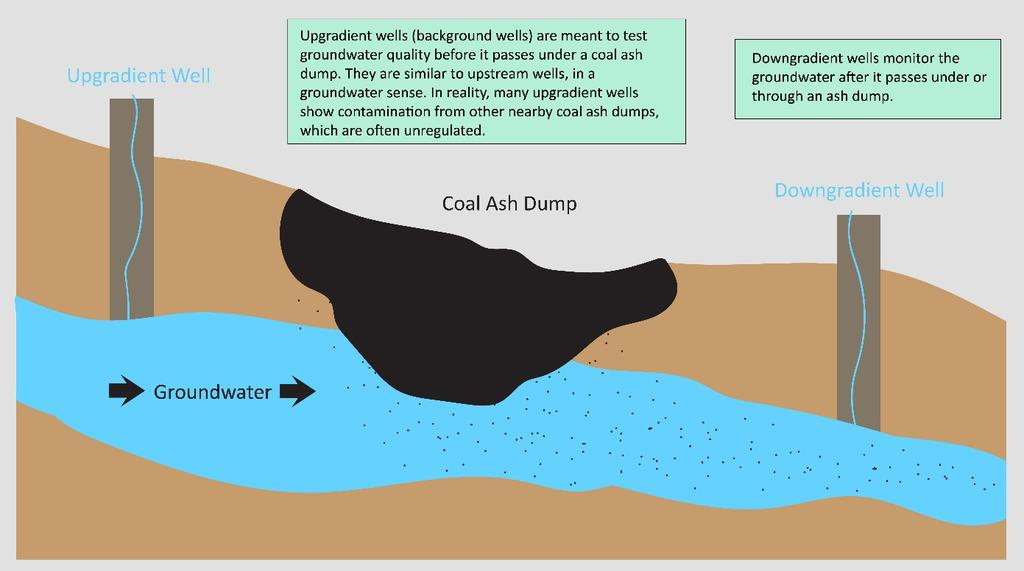
\includegraphics[width=1\linewidth]{figures/upgradientdowngradient} \caption{Difference Between Upgradient and Downgradient Wells}\label{fig:upgradientdowngradient}
\end{figure}

\begin{itemize}
\item
  upgradient wells (background wells) measures groundwater chemical
  levels BEFORE passing through a coal ash dump while downgradient wells
  monitor the groundwater AFTER it passes through an ash dump
\item
  we have reason to believe that many chemicals are NATURALLY OCCURING
  and as such, the statement made my environmental agencies regarding
  all groundwater being contaminated may be overstated
\item
  typically, we would estimate the amount of chemical contamination, for
  this example -- arsenic -- caused by a coal ash dump with the
  equation: downgradient arsenic concentration minus upgradient arsenic
  concentration
\item
  however, because there may be retired/unregulated upgradient wells
  that are occasionally contaminated already, this might be inaccurate
\end{itemize}

\begin{itemize}
\item
  END GOAL IS TO CORRECT THE CONTAMINATED VALUES
\item
  we have already conducted a preliminary investigation using a variety
  of machine learning techniques to aid us in identifying potential
  contaminated upgradient wells
\item
  we have also utilized bootstrapping and imputation techniques to
  correct for their measurements through by accounting for the innate
  contamination which may be caused by factors such as retired and
  unregulated wells
\item
  our methodologies have yet to account for another problem however,
  involving limit of detection problem which arises from the measuring
  devices' inability to obtain chemical concentrations smaller than a
  certain threshold amount
\end{itemize}

\hypertarget{data}{%
\subsection{Data}\label{data}}

\hypertarget{coalashrule}{%
\subsubsection{Coal Ash Rule}\label{coalashrule}}

\begin{itemize}
\item
  A large coal ash spill at the Tennessee Valley Authority (TVA) which
  occured on December 22, 2008 in Kingston, TN -- prompted the
  Environmental Protection Agency (EPA) to propose a set of standardized
  regulations and procedures to address the concerns regarding coal ash
  plants nationwide in the US {[}@Car2020{]}
\item
  This was known as the Coal Ash Rule, passed on December 19, 2014
  {[}@Car2020{]}
\item
  Changes were made to the Coal Ash Rule over the years in the form of
  `amendments,' one of which made required facility information and data
  to be made publicaly available to the public (April 15, 2015 rule
  change) {[}@Car2020{]}
\end{itemize}

\hypertarget{source-of-data}{%
\subsubsection{Source of Data}\label{source-of-data}}

\begin{itemize}
\item
  the data used in the study are from the results published in ``Annual
  Groundwater Monitoring and Corrective Action Reports'' which were made
  available to the public in March 2018 {[}@EIP2020{]}
\item
  these reports are in PDF format and are thousands of pages long, which
  makes it difficult for individuals to look through the data in a
  meaningful way {[}@EIP2020{]}
\item
  the EIP wranged the data into a more accessible machine-readable
  format which contains information from over 443 annual groundwater
  monitoring reports posted by 265 coal ash plants {[}@EIP2020{]}
\item
  they obtained the data from an online, publicly available database
  containing groundwater monitoring results from the first ``Annual
  Groundwater Monitoring and Corrective Action Reports'' in 2018 which
  was collected from coal plants and coal ash dumps under the Coal Ash
  Rule {[}@EIP2020{]}
\end{itemize}

\hypertarget{variables}{%
\subsubsection{Variables}\label{variables}}

\begin{itemize}
\item
  a coal ash site consists of multiple disposal areas
\item
  within these disposal areas lie multiple wells
\item
  each observation represents a well
\item
  wells are split into 2 different types - upgradient and downgradient
  wells
\item
  variables consist of information regard chemical contaminant
  concentrations and specifics regarding the well
\item
  from the 19 different contaminants (antimony, arsenic, boron, etc.
  \ldots) a major problem is that some wells only have measurements for
  certain chemicals and don't have them for others
\item
  we are currently using information from plants within illinois but
  there is data for all the states in the US
\end{itemize}

\end{document}
